\documentclass{article}

\usepackage{Vor2018skil}

\title{Tölvunarfræði 2, \semester \\ Skilaverkefni 11}
\author{}

\begin{document}
\maketitle
\hypersetup{pdftitle={Tölvunarfræði 2 - Skilaverkefni 11}}

Skila skal þessum verkefnum á \href{https://gradescope.com/courses/14122}{Gradescope}.

Þegar forriti er skilað inn til yfirferðar er mikilvægt að láta \textbf{niðurstöðurnar fylgja}. Öllum forritskóða skal skila framsettum með jafnbilaletri. Hann þarf að vera afritanlegur úr .pdf skjalinu. Vönduð framsetning og læsilegur kóði er hluti af verkefninu.

\question
Notið \texttt{DijkstraSP} úr algs4.jar á netið sem skilgreint er af skránni \href{https://algs4.cs.princeton.edu/43mst/mediumEWG.txt}{mediumEWG.txt}. Skrifið út fjarlægðir frá hnút númer 0 til hnúta númer 168, 200 og 201.

\paragraph{Athugasemd:} Beinagrind er ekki gefin, en dæmið er mjög stutt.

\question
Skjalið \href{https://raw.githubusercontent.com/Ernir/kennsluefni/master/T2/Code/w12/luxembourg.txt}{luxembourg.txt}\footnote{Uppruni: \url{http://www.math.uwaterloo.ca/tsp/world/countries.html}} inniheldur staðsetningar (hnit) á byggðakjörnum í smáríkinu Lúxemborg.

Gefum okkur nú að Lúxemborg vilji skipta út rafmagnsdreifikerfi sínu þannig að nýja kerfið myndi léttasta mögulega evklíðskt spanntré \eng{Euclidean minimum spanning tree} í neti sem myndað er út frá staðsetningunum. Þegar mynda skal slíkt tré lítum við á sem svo að mögulegt væri að bæta við legg á milli hverra tveggja hnúta (staðsetninga), þar sem þyngd leggsins er fjarlægðin á milli hnútanna.

Skrifið forrit í Java sem reiknar út léttasta evklíðska spanntré. Skilið kóðanum sem þið bætið við/breytið, myndinni sem þið fáið og þyngdinni sem forritið skrifar út. Frekari leiðbeiningar eru í \href{https://raw.githubusercontent.com/Ernir/kennsluefni/master/T2/Code/w12/EuclideanMST.java}{beinagrind}.

\paragraph{Ábending:} \texttt{luxembourg.txt} inniheldur endurtekningar sem þarf að hreinsa burt áður en teiknað er.

\begin{figure}[h]
	\caption{Hnitin í Lúxemborgar-netinu}
	\begin{center}
		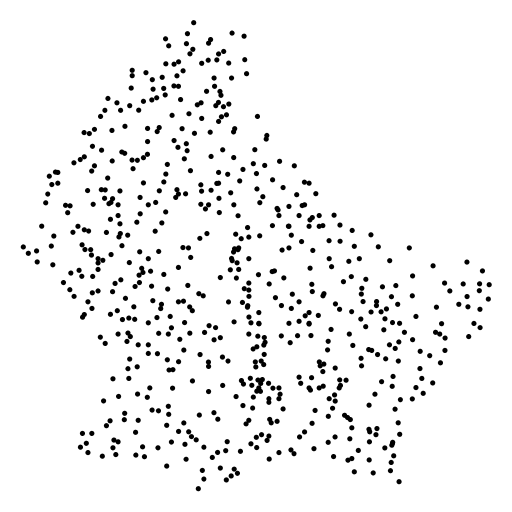
\includegraphics[width=0.7\textwidth]{luxembourg-points}
	\end{center}
\end{figure}

\begin{figure}
	\caption{Spanntré kennarans, með heildarþyngdina 10204.748738795975}
	\begin{center}
		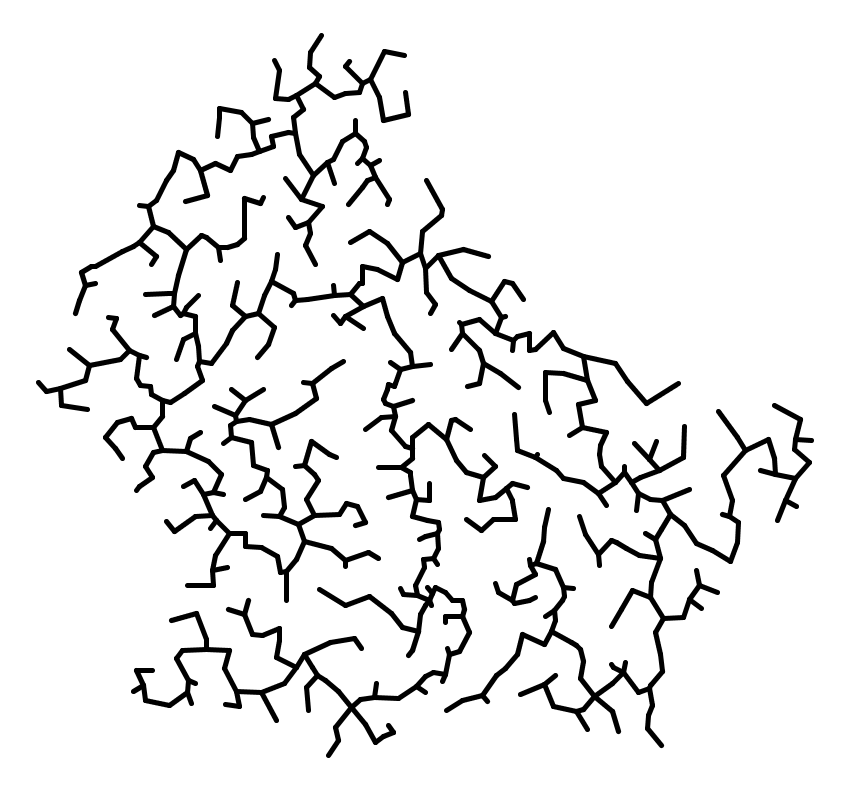
\includegraphics[width=0.7\textwidth]{luxembourg-mst}
	\end{center}
\end{figure}

\clearpage

\question

\href{https://en.wikipedia.org/wiki/Schulze_method}{Reiknirit Schulze} er kosningareiknirit sem vinnur á kjörseðlum þar sem kjósendur hafa tiltekið forgangsröðun á frambjóðendum.

Skrifið forrit sem les inn atkvæðaseðlana í \href{https://raw.githubusercontent.com/Ernir/kennsluefni/master/T2/Code/w12/votes.txt}{votes.txt} og skrifar út Schulze-sigurvegara kosningarinnar. Fyrsta lína skráarinnar táknar fjölda frambjóðenda. Hver hinna línanna táknar atkvæðaseðil, þar frambjóðendur eru auðkenndir með bókstöfum. Fyrsta val kjósandans er í fremsta dálki, annað val í 2. dálki, og svo koll af kolli.

Útgáfa af Floyd-Warshall reikniritinu sem hentar til útreikninga á sterkustu vegum fyrir Schulze er gefin í \href{https://raw.githubusercontent.com/Ernir/kennsluefni/master/T2/Code/w12/Schulze.java}{beinagrind}.

Skilið \texttt{main} fallinu sem þið skrifið sem og öllum hjálparaðferðum sem þið bætið við. Þegar forritið er rétt út fært á útskriftin að vera
\begin{center}
	\texttt{E > A > C > B > D}
\end{center} 
eða
\begin{center}
	\texttt{D < B < C < A < E}.
\end{center}

\paragraph{Frekari æfing:} Þó að beðið sé um lausn í Java hentar þetta verkefni vel til æfingar í C++. 

%\vfill
%
\includegraphics[width=0.5\linewidth]{hi-von-logo}

\end{document}